% Options for packages loaded elsewhere
% Options for packages loaded elsewhere
\PassOptionsToPackage{unicode}{hyperref}
\PassOptionsToPackage{hyphens}{url}
\PassOptionsToPackage{dvipsnames,svgnames,x11names}{xcolor}
%
\documentclass[
  letterpaper,
  DIV=11,
  numbers=noendperiod]{scrreprt}
\usepackage{xcolor}
\usepackage{amsmath,amssymb}
\setcounter{secnumdepth}{-\maxdimen} % remove section numbering
\usepackage{iftex}
\ifPDFTeX
  \usepackage[T1]{fontenc}
  \usepackage[utf8]{inputenc}
  \usepackage{textcomp} % provide euro and other symbols
\else % if luatex or xetex
  \usepackage{unicode-math} % this also loads fontspec
  \defaultfontfeatures{Scale=MatchLowercase}
  \defaultfontfeatures[\rmfamily]{Ligatures=TeX,Scale=1}
\fi
\usepackage{lmodern}
\ifPDFTeX\else
  % xetex/luatex font selection
\fi
% Use upquote if available, for straight quotes in verbatim environments
\IfFileExists{upquote.sty}{\usepackage{upquote}}{}
\IfFileExists{microtype.sty}{% use microtype if available
  \usepackage[]{microtype}
  \UseMicrotypeSet[protrusion]{basicmath} % disable protrusion for tt fonts
}{}
\makeatletter
\@ifundefined{KOMAClassName}{% if non-KOMA class
  \IfFileExists{parskip.sty}{%
    \usepackage{parskip}
  }{% else
    \setlength{\parindent}{0pt}
    \setlength{\parskip}{6pt plus 2pt minus 1pt}}
}{% if KOMA class
  \KOMAoptions{parskip=half}}
\makeatother
% Make \paragraph and \subparagraph free-standing
\makeatletter
\ifx\paragraph\undefined\else
  \let\oldparagraph\paragraph
  \renewcommand{\paragraph}{
    \@ifstar
      \xxxParagraphStar
      \xxxParagraphNoStar
  }
  \newcommand{\xxxParagraphStar}[1]{\oldparagraph*{#1}\mbox{}}
  \newcommand{\xxxParagraphNoStar}[1]{\oldparagraph{#1}\mbox{}}
\fi
\ifx\subparagraph\undefined\else
  \let\oldsubparagraph\subparagraph
  \renewcommand{\subparagraph}{
    \@ifstar
      \xxxSubParagraphStar
      \xxxSubParagraphNoStar
  }
  \newcommand{\xxxSubParagraphStar}[1]{\oldsubparagraph*{#1}\mbox{}}
  \newcommand{\xxxSubParagraphNoStar}[1]{\oldsubparagraph{#1}\mbox{}}
\fi
\makeatother


\usepackage{longtable,booktabs,array}
\usepackage{calc} % for calculating minipage widths
% Correct order of tables after \paragraph or \subparagraph
\usepackage{etoolbox}
\makeatletter
\patchcmd\longtable{\par}{\if@noskipsec\mbox{}\fi\par}{}{}
\makeatother
% Allow footnotes in longtable head/foot
\IfFileExists{footnotehyper.sty}{\usepackage{footnotehyper}}{\usepackage{footnote}}
\makesavenoteenv{longtable}
\usepackage{graphicx}
\makeatletter
\newsavebox\pandoc@box
\newcommand*\pandocbounded[1]{% scales image to fit in text height/width
  \sbox\pandoc@box{#1}%
  \Gscale@div\@tempa{\textheight}{\dimexpr\ht\pandoc@box+\dp\pandoc@box\relax}%
  \Gscale@div\@tempb{\linewidth}{\wd\pandoc@box}%
  \ifdim\@tempb\p@<\@tempa\p@\let\@tempa\@tempb\fi% select the smaller of both
  \ifdim\@tempa\p@<\p@\scalebox{\@tempa}{\usebox\pandoc@box}%
  \else\usebox{\pandoc@box}%
  \fi%
}
% Set default figure placement to htbp
\def\fps@figure{htbp}
\makeatother





\setlength{\emergencystretch}{3em} % prevent overfull lines

\providecommand{\tightlist}{%
  \setlength{\itemsep}{0pt}\setlength{\parskip}{0pt}}



 


\KOMAoption{captions}{tableheading}
\makeatletter
\@ifpackageloaded{bookmark}{}{\usepackage{bookmark}}
\makeatother
\makeatletter
\@ifpackageloaded{caption}{}{\usepackage{caption}}
\AtBeginDocument{%
\ifdefined\contentsname
  \renewcommand*\contentsname{Table of contents}
\else
  \newcommand\contentsname{Table of contents}
\fi
\ifdefined\listfigurename
  \renewcommand*\listfigurename{List of Figures}
\else
  \newcommand\listfigurename{List of Figures}
\fi
\ifdefined\listtablename
  \renewcommand*\listtablename{List of Tables}
\else
  \newcommand\listtablename{List of Tables}
\fi
\ifdefined\figurename
  \renewcommand*\figurename{Figure}
\else
  \newcommand\figurename{Figure}
\fi
\ifdefined\tablename
  \renewcommand*\tablename{Table}
\else
  \newcommand\tablename{Table}
\fi
}
\@ifpackageloaded{float}{}{\usepackage{float}}
\floatstyle{ruled}
\@ifundefined{c@chapter}{\newfloat{codelisting}{h}{lop}}{\newfloat{codelisting}{h}{lop}[chapter]}
\floatname{codelisting}{Listing}
\newcommand*\listoflistings{\listof{codelisting}{List of Listings}}
\makeatother
\makeatletter
\makeatother
\makeatletter
\@ifpackageloaded{caption}{}{\usepackage{caption}}
\@ifpackageloaded{subcaption}{}{\usepackage{subcaption}}
\makeatother
\usepackage{bookmark}
\IfFileExists{xurl.sty}{\usepackage{xurl}}{} % add URL line breaks if available
\urlstyle{same}
\hypersetup{
  pdftitle={tesis-filo},
  pdfauthor={Jaime Vergara Sanfuentes},
  colorlinks=true,
  linkcolor={blue},
  filecolor={Maroon},
  citecolor={Blue},
  urlcolor={Blue},
  pdfcreator={LaTeX via pandoc}}


\title{tesis-filo}
\author{Jaime Vergara Sanfuentes}
\date{2025-03-05}
\begin{document}
\maketitle

\renewcommand*\contentsname{Table of contents}
{
\hypersetup{linkcolor=}
\setcounter{tocdepth}{2}
\tableofcontents
}

\bookmarksetup{startatroot}

\chapter{Index}\label{index}

{/00} The epoch of the immen-city

Issue No.~0July 2025

AuthorJaime Vergara Sanfuentes

Index

Chapter 1

Chapter 2

Chapter 3

Chapter 4

Chapter 5

Chapter 6

References

\bookmarksetup{startatroot}

\chapter{The modern inmensity of the
urban}\label{the-modern-inmensity-of-the-urban}

\bookmarksetup{startatroot}

\chapter{\texorpdfstring{{/01} The modern inmensity of the
urban}{/01 The modern inmensity of the urban}}\label{the-modern-inmensity-of-the-urban-1}

figure 1. Built up properties between 1820 - 2000 \footnote{Uhl,
  Johannes H. (2020)}

figure 2. Variation over 5-year intervals in built-up properties between
1820--2000 \footnote{United Nations, Department of Economic and Social
  Affairs. (2019)}

\begin{figure}

\centering{

\pandocbounded{\includegraphics[keepaspectratio]{figures/chap_1_fig_3_global_building_atlas_heigth_maps.jpg}}

}

\caption{\label{fig-gba-overview}}

\end{figure}%

figure 3. Global and complete dataset of building polygons, heights and
LoD1 \footnote{United Nations, Department of Economic and Social
  Affairs. (2019)}

In pre-modern times, our relationship with the urban environment could
be engaged---if not directly manipulated---through simple pedestrian
locomotion. Wandering served as a sufficient means to experience and
intuitively assimilate the urban tissue, and also to design its
intervention. If we should put the scale of the historical city under
the taxonomy presented by Stolk and Portugali (2016)\footnote{Stolk, E.,
  \& Portugali, J. (2016)}, we could classify it as an environmental
scale: an order of magnitude where the user and designer can be
subjected to the whole of urban's perceptual cues over time.

As cities expanded, their immense scale began to represent more than
just a practical complication of transport; it signaled an ontological
withdrawal of the urban phenomenon and an epistemological shift toward
-at that moment in history- highly abstract ways of conceiving the city.
This scale rendered the ecology of the premodern city unviable simply by
decoupling our lives from the territory by means of distance. Indeed the
proportions of urban growth are overwhelming, both demographically and
spatially. After reaching a population of 500 million in 1543, it took
nearly seven centuries (260 years) to reach one billion in 1803. From
that point forward, the pace accelerated: 125 years later, in 1928, the
population doubled to two billion; and merely 47 years after that, in
1975, it surpassed four billion. In less than half a century, the figure
quadrupled. By 2024, we have already surpassed 8 billion, and
projections indicate that before 2100, we will reach between 10 and 11
billion.

The growth that transformed the city of the past century into a
megalopolis---and which, according to Doxiadis (1969), is poised to
finally nest the ecumenopolis in the centuries to come---drew the urban
phenomenon to a scale where the information overwhelmed our capacity to
retrieve meaning from it (Portugali, 2016)\footnote{Portugali, J. (2016)},
producing the sensation of a noisy or simply `trash' urban environment.
The immense object that our cities have become is what we could classify
as a geographic object, which, according to Stolk and Portugali
(2016)\footnote{Stolk, E., \& Portugali, J. (2016)}, is no longer
relatable in time. Thus, the `citizen as a whole' relating to a singular
urban environment does not exist anymore.

But as the city change our relation to the urban environment also did.
The technological evolution of transport (cars, trains, and planes)
alongside remote sensing (satellite imaging, geopositioning systems, and
surveying equipment) allowed citizens to maintain a relationship with
the immense urban environment. By drastically reducing the time required
to traverse the city and providing a bird's-eye representation of our
position, these tools kept us related to the urban environment to the
cost of accepting a discontinuous locomotion and interface that
fractures our perception of the urban landscape.

The urban environment now enters our lives only partially, closer to the
climate and other worldly events. Even with the technological
advancements of the twentieth century, relating to the totality of the
urban landscape through intuition has become psychologically difficult
to develop. The effects are clear: the loss of the capacity to relate to
it through an immediate, singular representation generated by
sensibility (Kant, 1781)\footnote{Kant, I. (1998)} has pushed design
mediums toward abstraction.

Although its distance could invite us to think that the urban landscape
is not relevant to the locality of our lives, Henri Lefebvre would argue
that the local cannot be defined tautologicaly without the global, and
that globalisation would not develop itself from the local spaces were
its concretises Fondation Gabriel Péri. (2022)\footnote{Fondation
  Gabriel Péri. (2022)}. Consequently sensing the mode through which we
relate to the urban landscape, reveals the societal need of inhabiting
the immensity of the modern city.

What precisely was lost during this ontological withdrawal of the city?
If the modern metropolis can no longer be apprehended through intuition,
upon what technologies was it constructed to manage the production of
the modern urban environment? To what extent do the triumphant
methodologies that concretize the modern urban landscape overcome the
problem of immensity? Finally, how might we trace a genealogy of
embodied design methodologies aimed at bypassing this abstraction to
reclaim an intuitive connection to the urban environment?

Index

Chapter 1

Chapter 2

Chapter 3

Chapter 4

Chapter 5

Chapter 6

References

Footnotes

\bookmarksetup{startatroot}

\chapter{What happens to urban
landscaping?}\label{what-happens-to-urban-landscaping}

\bookmarksetup{startatroot}

\chapter{\texorpdfstring{{/02} What happens to urban
landscaping?}{/02 What happens to urban landscaping?}}\label{what-happens-to-urban-landscaping-1}

The methods through which urbanism operated, inherited from its mother
discipline architecture, became obsolete as the design medium upon which
it based its concretization became increasingly maladjusted to the scale
of the environment.

For architecture, this crisis, produced by the sheer immensity of the
city, was characterized by an increasing ``regime of complexity''
\footnote{Koolhaas, R. (1995).} that rendered insufficient pre-modern
concrete design media (profiles, cuts, plans, perspectives, constructive
terms). Designing at an experienceable scale handed the design process
from a close relation with the artifacts, where the concretization of
the urban could be surveyed and designed from perceptual cues that came
directly from the experience of the urban environment, to one where
design based itself on a tabular and cartographic disassembly corpus of
the urban environment.

For this discipline, tightly related to the perception and experience of
space, the new immensity of the urban tissue was viewed by some authors
as catastrophic. In the 1970s, Lefebvre (1972) \footnote{Lefebvre, H.
  (1972).} noted that at that point, an epistemology of what the city
had become did not even exist. Famously and polemically noted by Rem
Koolhaas in his essay on urbanism, the crisis was qualified as a
``collective shame'' and a ``crater of our understanding of the modern
city'' \footnote{Koolhaas, R. (1995).}.

According to Koolhaas (1995) \footnote{Koolhaas, R. (1995).}, the
inability to concretely represent the `problem of bigness' within the
urban environment remains a largely ignored subject of research.
Nevertheless, the epistemological challenge posed by massive scale is an
ancient one. The anekantavada, the famous Jainist parable of the blind
men and the elephant, encapsulates this dilemma: as each man observes
only a localized fraction of the animal, they interpret their isolated
experience as an entirely different entity---one sees the trunk as a
snake, another the leg as a pillar, and the tail as a lion; all fail to
share a sense of the beast as a whole.

Within modern planning rationale, the fragmented perspectives of the
parable find their equivalent in what De Roo (2016) \footnote{De Roo, G.
  (2016).} defines as the relativist approach to planning. Relativism,
in this context, refers to the subjective worlds of meaning that emerge
as individuals develop, exchange, and incorporate mentally constructed
values. In this rationale, the human experience of the city is mapped as
a synergetic Inter-Representation Network, where the individual urban
agents comprising that network share only external representations of
the phenomena. The analysis of this network shows it is fundamentally
constrained by the biological dimensions of the agents' sensory
receptors and the finite capacity of their motor effectors to process,
convey, and manipulate the immensity of their urban experiences.

Producing from this perspective, and even planning a technical object,
devolves forcefully into abstraction. This rationale allows for an
experience of the urban that can only be conceived through an abstract,
collective reservoir of memories and not shared experience.

While a shared reservoir of memories is defined by its relation to an
external representation of the urban tissue, a shared experience relies
on an intuitive, sensory relation to the urban environment and its
inhabitants. By relying purely on abstraction, urban design is completed
by imagination into utopic projects---projects which, much like the
monstrous elephant in the Indian parable, are fantastic projections of
the designer.

Due to the loss of sensibility over the urban landscape, what emanates
through our partial perspective is a sense of extension devoid of
meaning, colloquially termed `junkspace' by Koolhaas (2002) \footnote{Koolhaas,
  R. (2002).}.

The parable of the Indian elephant reveals that this immensity is
perceived to be outside of our Umwelt, which von Uexküll (1934/1957)
\footnote{von Uexküll, J. (1957).} defines as the lived sensory
environment of the citizen. However, the complexity of the problem lies
not only in the effectors but also in the actuators of our behavior
vis-à-vis urban beings. As concepts deprived of sensibility are void,
the epistemological crisis of immensity can be typified as a failure in
the cognitive capacity to synthesize the urban landscape.

From a design perspective, a crisis in the concretization of urban
ideations translates directly into the designer's inability to relate to
the urban landscape. Becoming an `irresponse-able' individual
\footnote{Kousoulas, S., \& Radman, A. (2026).}, the designer produces
and plans things to which they cannot relate. Consequently, as the scale
challenges representation, designers develop difficulties expressing
geographic thoughts within their design medium, unleashing actions upon
the urban landscape that cannot be fully appreciated by the very
designers who effectuated them.

The loss of form described above carries severe implications for the
modern epoch, with dire consequences for the creative endeavor at the
geographic scale. Viewed from a classical philosophical perspective, the
lack of synthesis over the landscape marks a deterrence in our capacity
for the creation of urban beings---its poiesis. Without bounds to the
underlying form or eidos \footnote{Aristotle. (1984).}, two
dysfunctional creative dispositions emerge:

On the one hand, creation devoid of form produces a fragmented
objectification of the urban fabric that devolves into mindless
relations to the built environment without any unifying civic idea,
sprawling into modern vernacular architecture.

On the other hand, forms devoid of creation tend toward utopian master
plans that retreat entirely from the concrete production of the living
urban tissue, taking refuge in pure geometry and abstract technologies.

For Louis Kahn (1969), creating without the measurable---which he
equates to light---relegates architecture to the unmeasurable realm of
Silence, an entirely imaginary and unmanifested exercise. The
measurable, structurally aligned with the techne in architecture,
constitutes the active medium through which light is spent to bring
material beings into existence. Without the technical capacity to cast
light into matter, buildings remain ontologically incomplete,
manifesting either as unrealized abstractions or as monstrous
materializations.

The art of architecture, therefore, requires dominion over technique to
actualize entities endowed with a final cause (telos). Stripped of this
teleological imperative, the twentieth-century urban landscape provoked
a profound disciplinary anxiety: the fear that art would retreat from
the discipline entirely. As this retreat materialized---a phenomenon
diagnosed by Koolhaas (1995) \footnote{Koolhaas, R. (1995).}---pure
technique assumed control. The concretization of matter proceeded driven
solely by the blind momentum of its efficient causes, or retreated into
empty, meaningless geometries (pure eidos) \footnote{Aristotle. (1984).}.
This epistemological collapse necessitates a subsequent historical
inquiry: what were the specific abstract technologies that usurped the
production of the city during this architectural retreat?

\pandocbounded{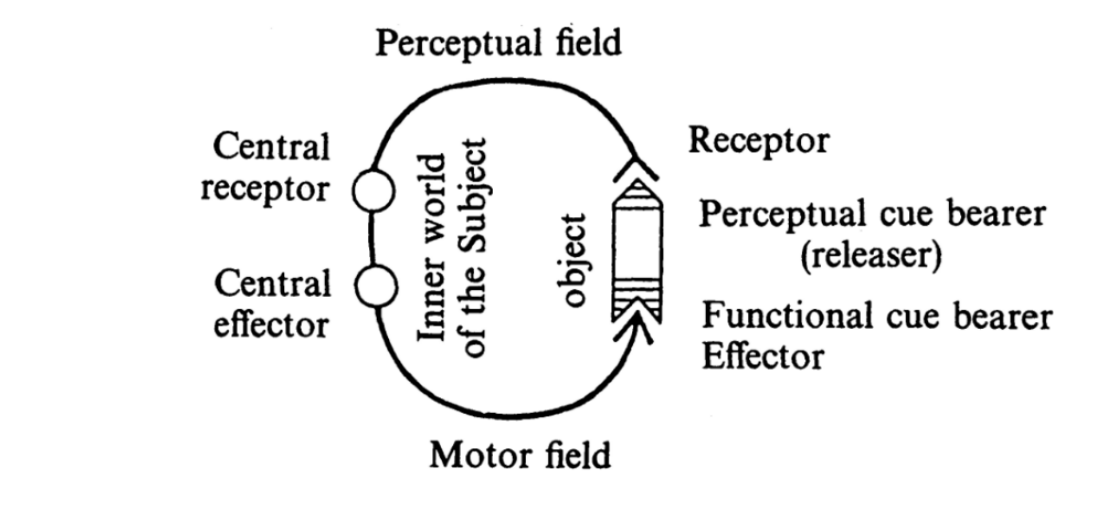
\includegraphics[keepaspectratio]{figures/chap_2_fig_3_three_synergetic_inter_representationfuncional_cycle.png}}

figure 1. Funcional cycle \footnote{von Uexküll, J. (1957).}

\pandocbounded{\includegraphics[keepaspectratio]{figures/chap_2_fig_1_blind_men_and_the_elephant.png}}

figure 2. Blind men and the elephant, 1907 American illustration.
\footnote{Blind men and the elephant {[}Illustration{]}. (1907).}

\pandocbounded{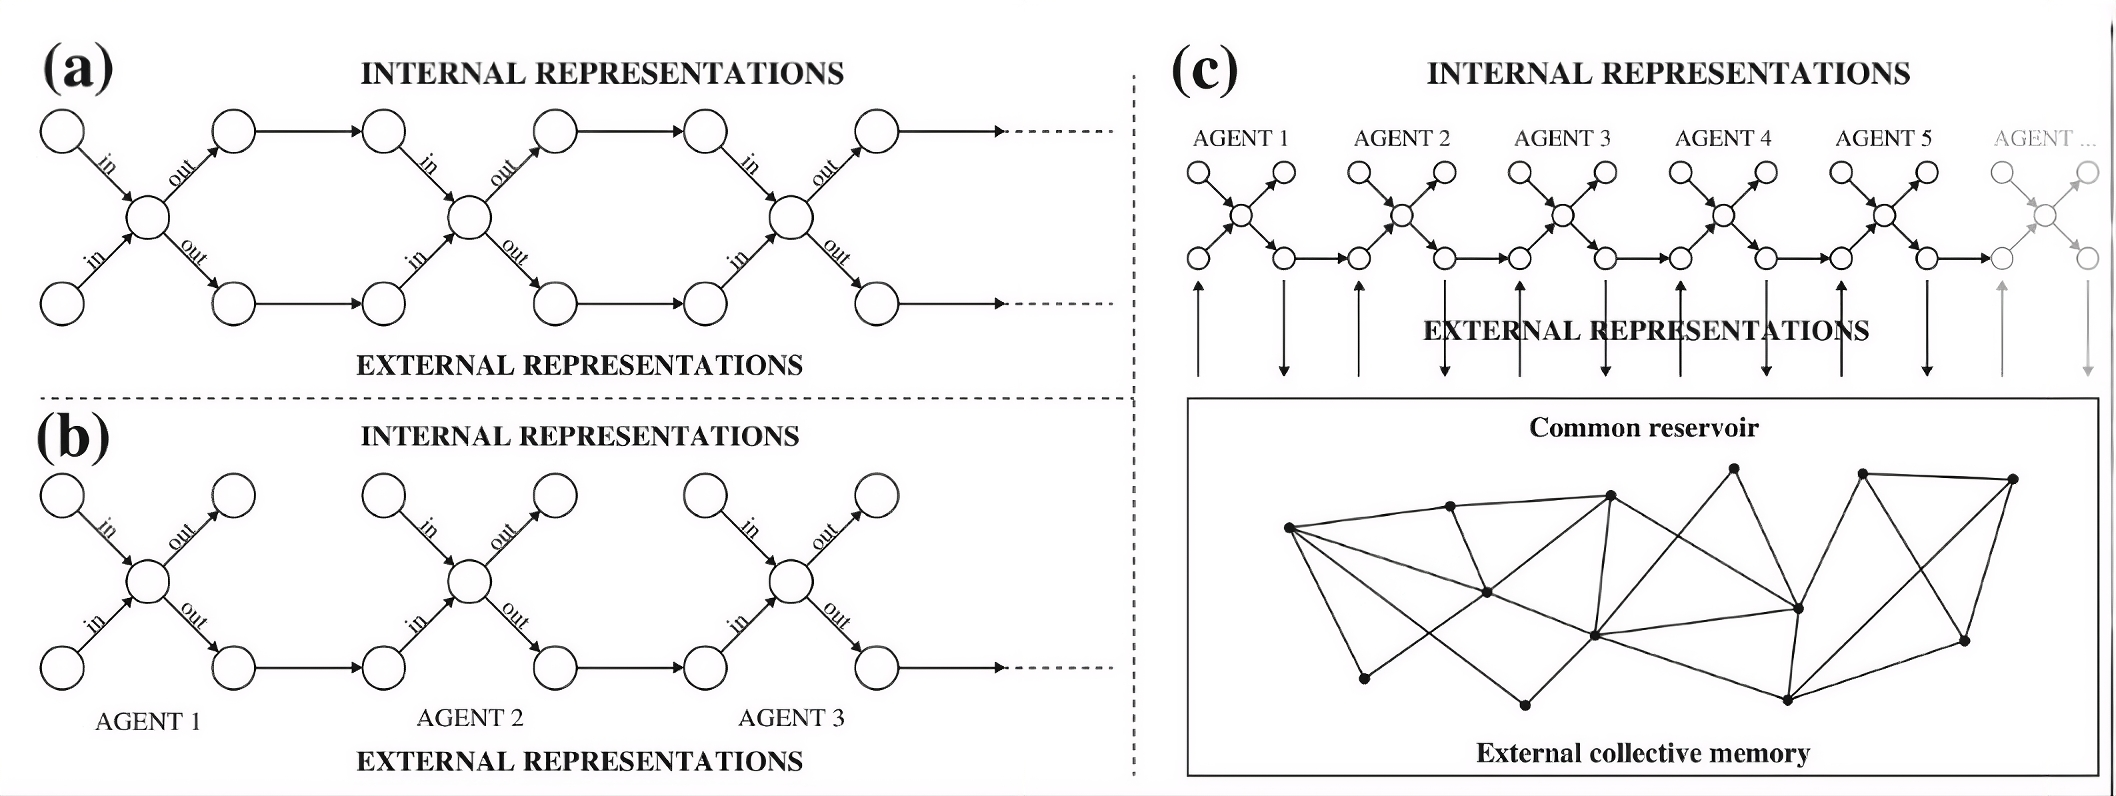
\includegraphics[keepaspectratio]{figures/chap_2_fig_2_three_synergetic_inter_representation.png}}

figure 3. Three Synergetic Inter-Representation Network sub models
\footnote{Stolk, E., \& Portugali, J. (2016).}

\pandocbounded{\includegraphics[keepaspectratio]{figures/chap_2_fig_4_primitive_hut.png}}

figure 4. Primitive hut \footnote{Eisen, C. (1755).}

Index

Chapter 1

Chapter 2

Chapter 3

Chapter 4

Chapter 5

Chapter 6

References

Footnotes

\bookmarksetup{startatroot}

\chapter{The experimental disposition of the urban
production}\label{the-experimental-disposition-of-the-urban-production}

\bookmarksetup{startatroot}

\chapter{\texorpdfstring{{/03} The experimental disposition of the urban
production}{/03 The experimental disposition of the urban production}}\label{the-experimental-disposition-of-the-urban-production-1}

\pandocbounded{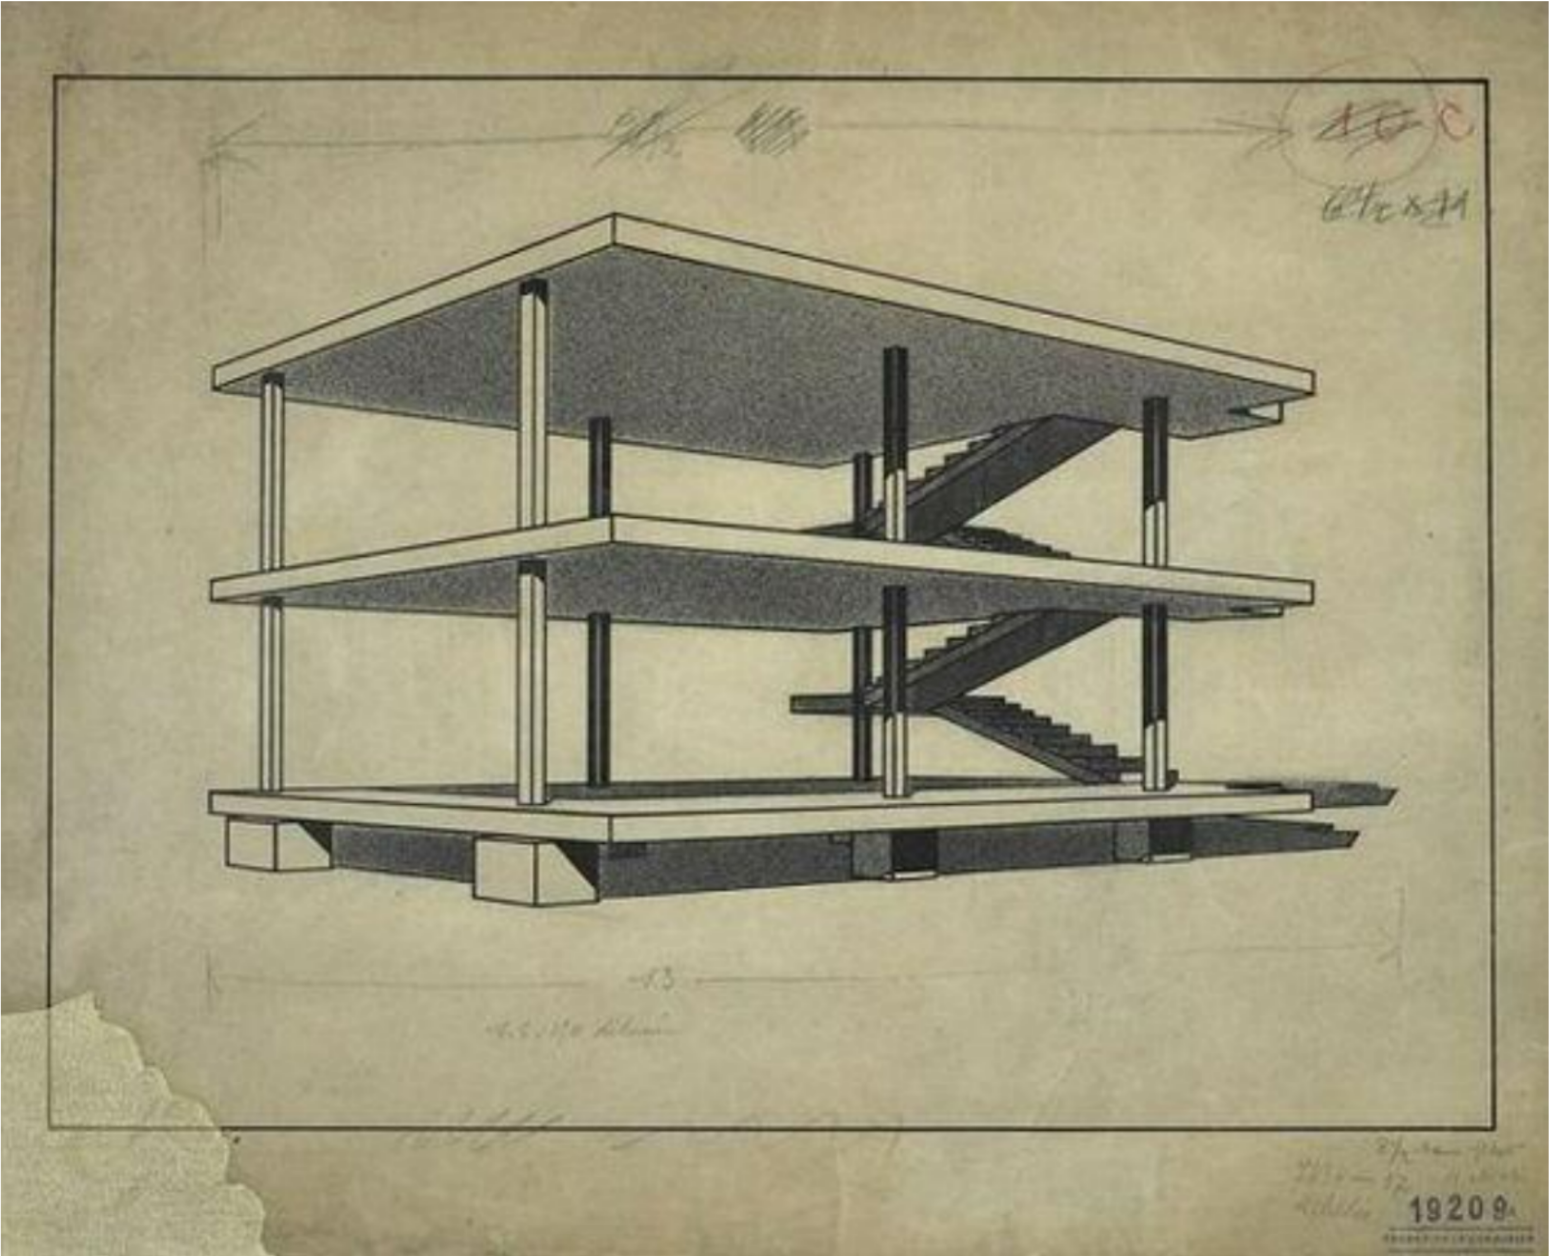
\includegraphics[keepaspectratio]{figures/chap_3_fig_1_la_maison_domino_le_corbusier.png}}

figure 1: La maison Domino, Le Corbusier 1914-1915 \footnote{Le
  Corbusier. (1914).}

\pandocbounded{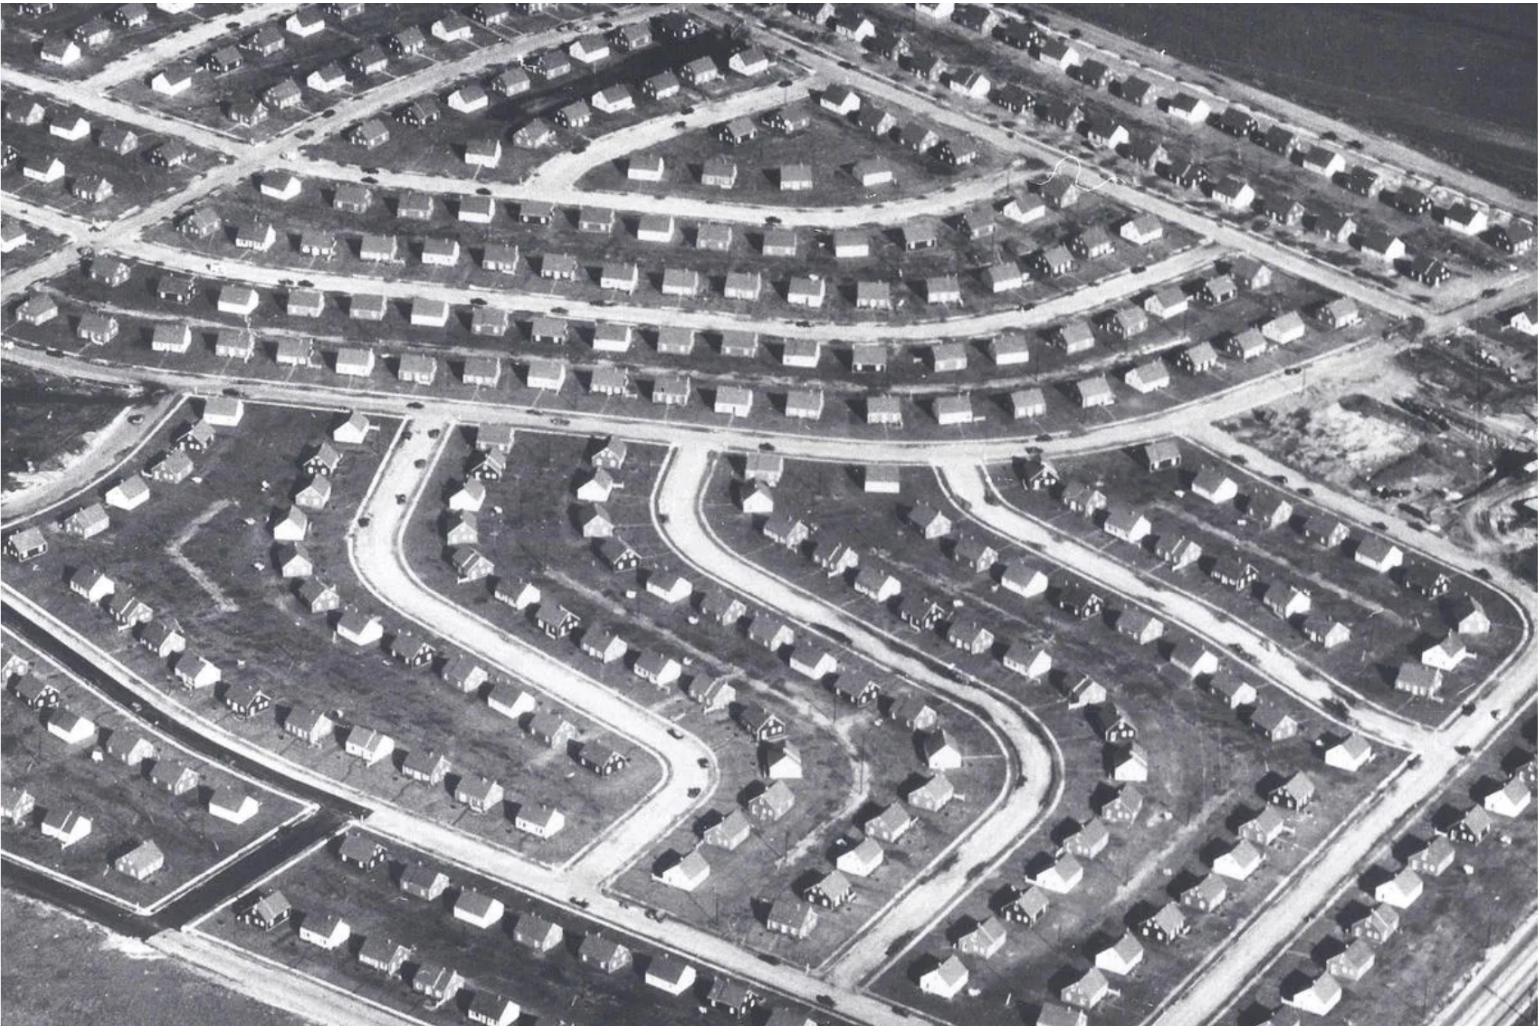
\includegraphics[keepaspectratio]{figures/chap_3_fig_2_early_capes_aerial_view_of_levittown.png}}

figure 2: Early Capes Aerial View of Levittown \footnote{Levittown
  library. (1950).}

\pandocbounded{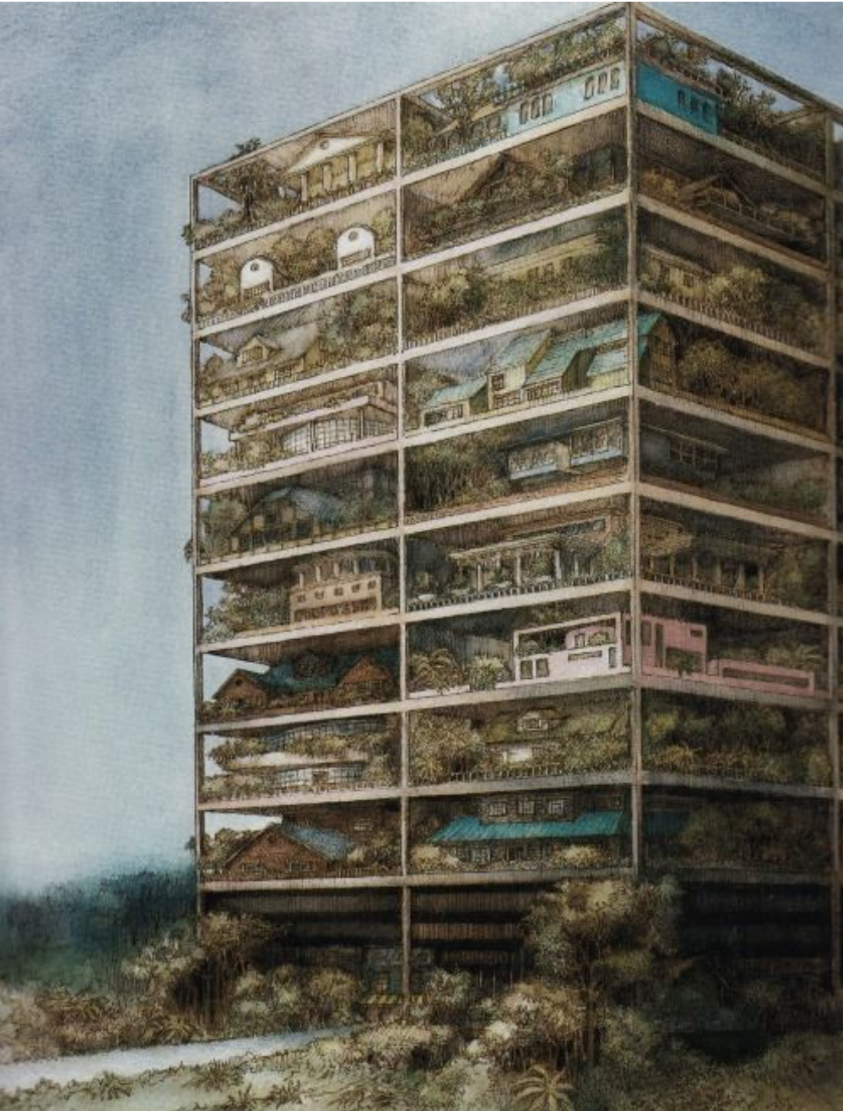
\includegraphics[keepaspectratio]{figures/chap_3_fig_3_highrise_of_houses_SITE_1981.png}}

figure 3: Highrise of houses, SITE 1981 \footnote{SITE (1981).}

Design mediums that adapted to this new magnitude of the city relied
heavily on science and technique, and would belong if we situated them
in the cognitive capabilities of design elaborated by Roo (2016)
\footnote{De Roo, G. (2016).} in an objectivist pole. The project of
scientifically approaching the city drove various disciplines to produce
the urban environment through what Heidegger, M. (1977) \footnote{Heidegger,
  M. (1977).} would term an 'experimental disposition.

By producing urban elements in absolute isolation and subsequently
injecting them into the urban environment from an abstract perspective,
the scientific production, embodied in the management philosophy of
Fordism and Taylorism, concretise the city by means of sterilization of
its production from any relation that was not planned.

The concretization of the urban tissue became then possible only through
the decomposition of designed artifacts into discrete parts---parts that
revealed increasingly precise, that could be manufactured into an
isolated industrial chain.

Another key element of the concretization of the modern urban landscape
is the circumscription of domains of the urban into parcels. With this
last link, the enterprise could, in anticipatory form, define the space
that the urban beings were they would be concretised into the city.

The production of this urban landscape from a technological standpoint
would engulf a strange paradox in the reading of Simondon (1958/2017)
\footnote{Simondon, G. (2017).}. As abstract objects are defined by
their degree of freedom from the environment, the experimental device of
the modern epoch would have somehow allowed abstraction to be placed
over the environment. By means of isolation, it would have allowed the
concretisation of a city of abstract parcels, each one with internal
relations.

The elementarization of the city, achieved through this experimental
disposition, was effectuated across several disciplinary domains. The
most notable producers of the modern city---though by no means the only
ones---were disciplines such as engineering and economics, which built
vast, objective fields for measuring the design of the urban
environment.

Nevertheless, this modern enterprise did not concern itself with the
intuition that we could develop with the globality of the urban
environment. Indeed, factors that would compromise the hermeticity of
the chain of production, such as pre-existences or the complexity of the
citizen, were destroyed or set aside in favor of a blank slate or
canvas.

This established a strict realist perspective in city design: an
approach that measures objective, quantifiable relations within the
environment while failing to account for the human elements of its lived
use (De Roo, 2016) \footnote{De Roo, G. (2016).}.

Index

Chapter 1

Chapter 2

Chapter 3

Chapter 4

Chapter 5

Chapter 6

References

Footnotes

\bookmarksetup{startatroot}

\chapter{Experiences of the modern urban
landscape}\label{experiences-of-the-modern-urban-landscape}

\bookmarksetup{startatroot}

\chapter{\texorpdfstring{{/04} Experiences of the modern urban
landscape}{/04 Experiences of the modern urban landscape}}\label{experiences-of-the-modern-urban-landscape-1}

It was Le Corbusier who, as early as Vers une architecture (1923),
translated this objective rationale directly into architecture. By
decomposing the conditions of inhabitation into components, he famously
dreamt of mass-producing houses the way industry manufactured cars
\footnote{Le Corbusier. (1923).}. He put forward the modernist vision of
the `machine for living', a technological project of building an
habitational unit. synergized with the industrialization of
construction, driving the development of concrete formwork, sheet metal,
steel structural modules, and advanced insulation technologies. The
genealogy uniting modern architecture with industrialization meant that
construction techniques were fully adapted to this elementarization of
the aspect of human life, a sort of life support as Sloterijk. (2016)
\footnote{Sloterdijk, P. (2016).}.

The legacy of Le Corbusier's habitational units ---and their conceptual
roots in the localized efficiency of the automobile ---has fundamentally
configured our experience of the modern urban fabric. Through capsular
transit and the development of life-supported spatial enclosures, the
locomotion barriers and sheer immensity imposed by the geographic scale
can finally be managed. The proliferation of these technical spheres
that envelop us constitutes one of the most defining characteristics of
the contemporary urban environment. As François Ascher asserts, the
order of the modern metropolis relies heavily on its capacities for
storage, logistics, and isolation \footnote{Fabian Alvarado David.
  (2016).}. Consequently, everyday technologies---such as refrigerators,
air conditioners, electrical outlets, polarized windows, and
free-flowing highways---act as crucial prosthetic devices to preserve
the co-isolation that configures our urban life. These technologies
actively configure the deterritorialized, insulated relationship we now
maintain with the broader urban environment.

Within this encapsulating foam, geographic scale loses its immediate
relevance. Much like the weather outside a well-built home is rendered
inconsequential to its inhabitants, we have technologically disengaged
our daily lives from the sheer immensity of the city. The ordinary
experience of the urban tissue no longer requires a sustain itself in
physical confrontation with its overall aspect. Moreover, design of the
urban environment absolutely seem to demand it in order to orchestrate
the geography of the urban landscape.

Many times under hodology, the foamy experience of the modern city
organizes its logistics through a discontinuity between states of
movement and inertia, where movement attempts, through the means of
velocity, to overcome the logistic challenges of physical distances. As
Koolhaas mentions, this discontinuity takes the maximum architectural
form of what we could call, in terms of topological features, nodes of
maximum degree of connection. From the logic of the hyperlink, through
the suspensive space of the elevator, to the enormous hub-and-spoke
terminals of airports, the modern city landscape reveals itself through
the triumphant genealogy of machines to inhabit movement.

Through speed and life-support systems, modern technology has pushed the
utopia that immensity could be inhabited through instantaneity. Many
abstract technologies have been devised by science fiction to finally
split the existence in motion from that of stillness. While science
fiction has long devised abstract technologies to permanently bifurcate
existence into absolute motion and absolute stillness---such as the
teleporter of Star Trek or the hyperdrive of Star Wars---the project of
inhabiting `bigness' has driven contemporary geography and technical
genealogies toward the exact same binary division of the world.

figure 1. Mickey's trailer \footnote{Sharpsteen, B. (1938).}

\pandocbounded{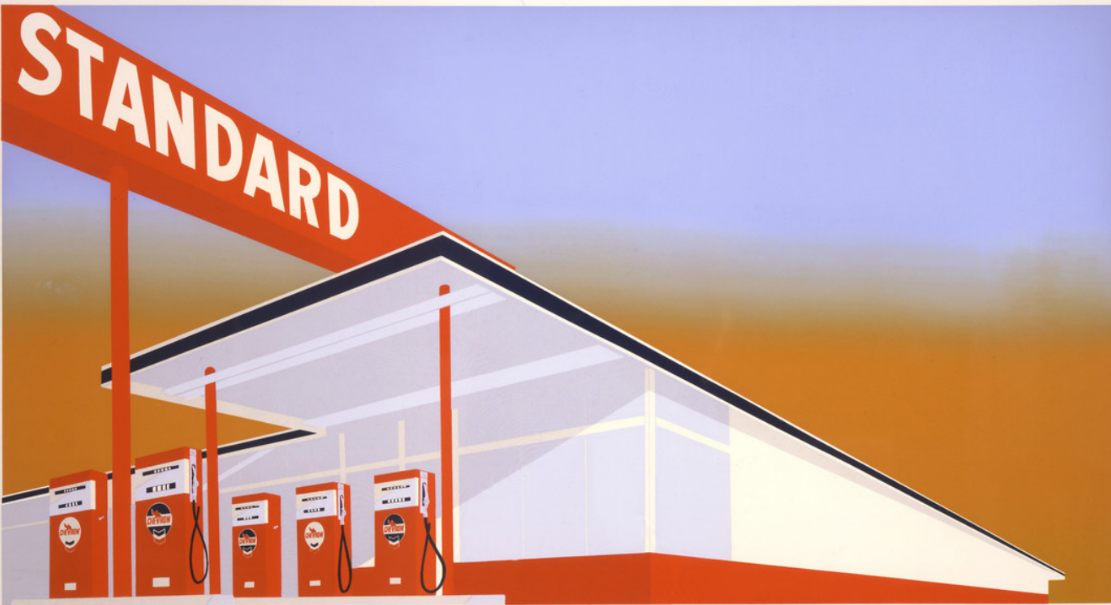
\includegraphics[keepaspectratio]{figures/chap_4_fig_2_standard_station_Ed_ruscha_(1966).png}}

figure 2. Standard Station, Ed Ruscha (1966) \footnote{Ed Ruscha (1966).}

\pandocbounded{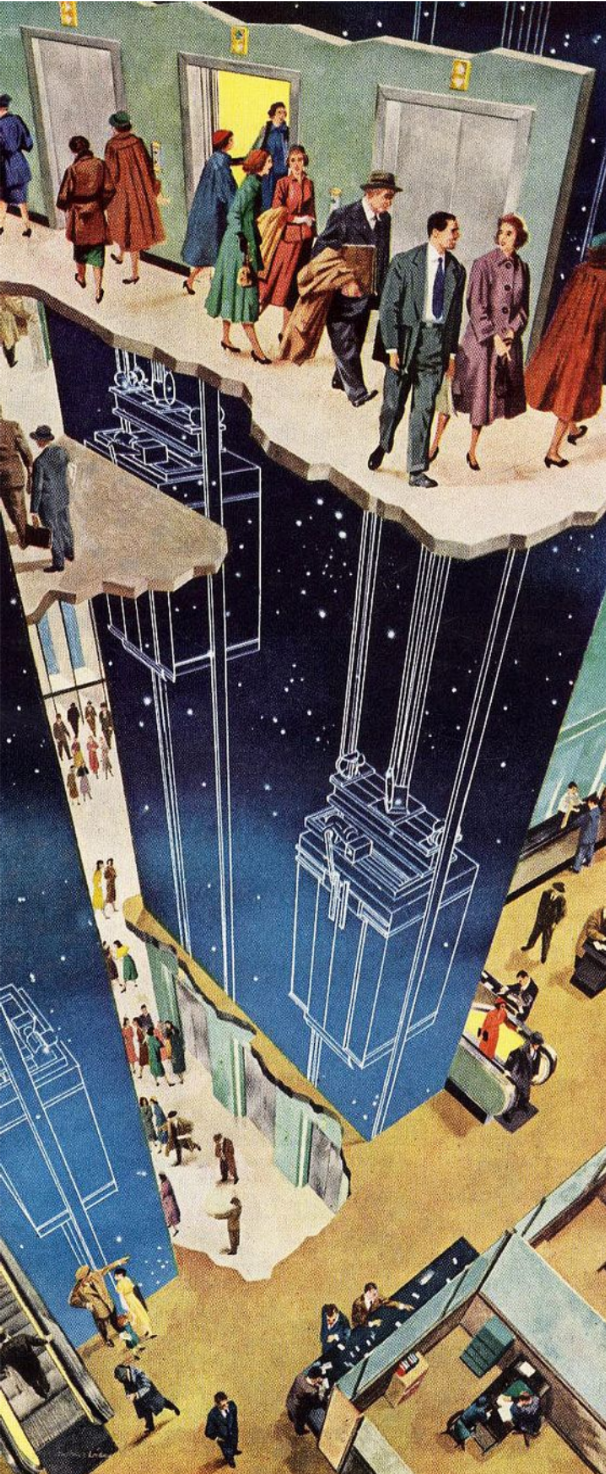
\includegraphics[keepaspectratio]{figures/chap_4_fig_3_the_tenants_think_it_s_wonderful_otis_1952.png}}

figure 3. The tenants think it's wonderful, Otis 1952 \footnote{Otis
  Elevator Company. (1952).}

Index

Chapter 1

Chapter 2

Chapter 3

Chapter 4

Chapter 5

Chapter 6

References

Footnotes

\bookmarksetup{startatroot}

\chapter{The geodesic enterprise and the production of the image of the
world}\label{the-geodesic-enterprise-and-the-production-of-the-image-of-the-world}

\bookmarksetup{startatroot}

\chapter{\texorpdfstring{{/05} The geodesic enterprise and the
production of the image of the
world}{/05 The geodesic enterprise and the production of the image of the world}}\label{the-geodesic-enterprise-and-the-production-of-the-image-of-the-world-1}

\pandocbounded{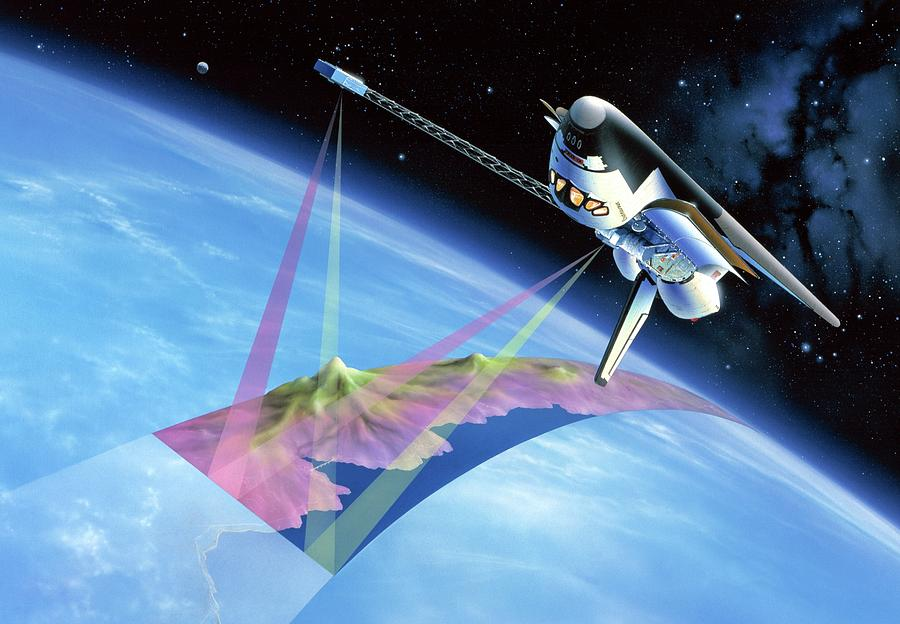
\includegraphics[keepaspectratio]{figures/chap_5_fig_1_shuttle_nasa_topography_mission_1999.jpg}}

figure 1: Shuttle Nasa Topography Mission (SRTM) (1999) \footnote{Shuttle
  Nasa Topography Mission (SRTM) (1999)}

figure 2: Google Earth Studio. (2018) Animation Reel \footnote{Google
  Earth. (2018).}

\pandocbounded{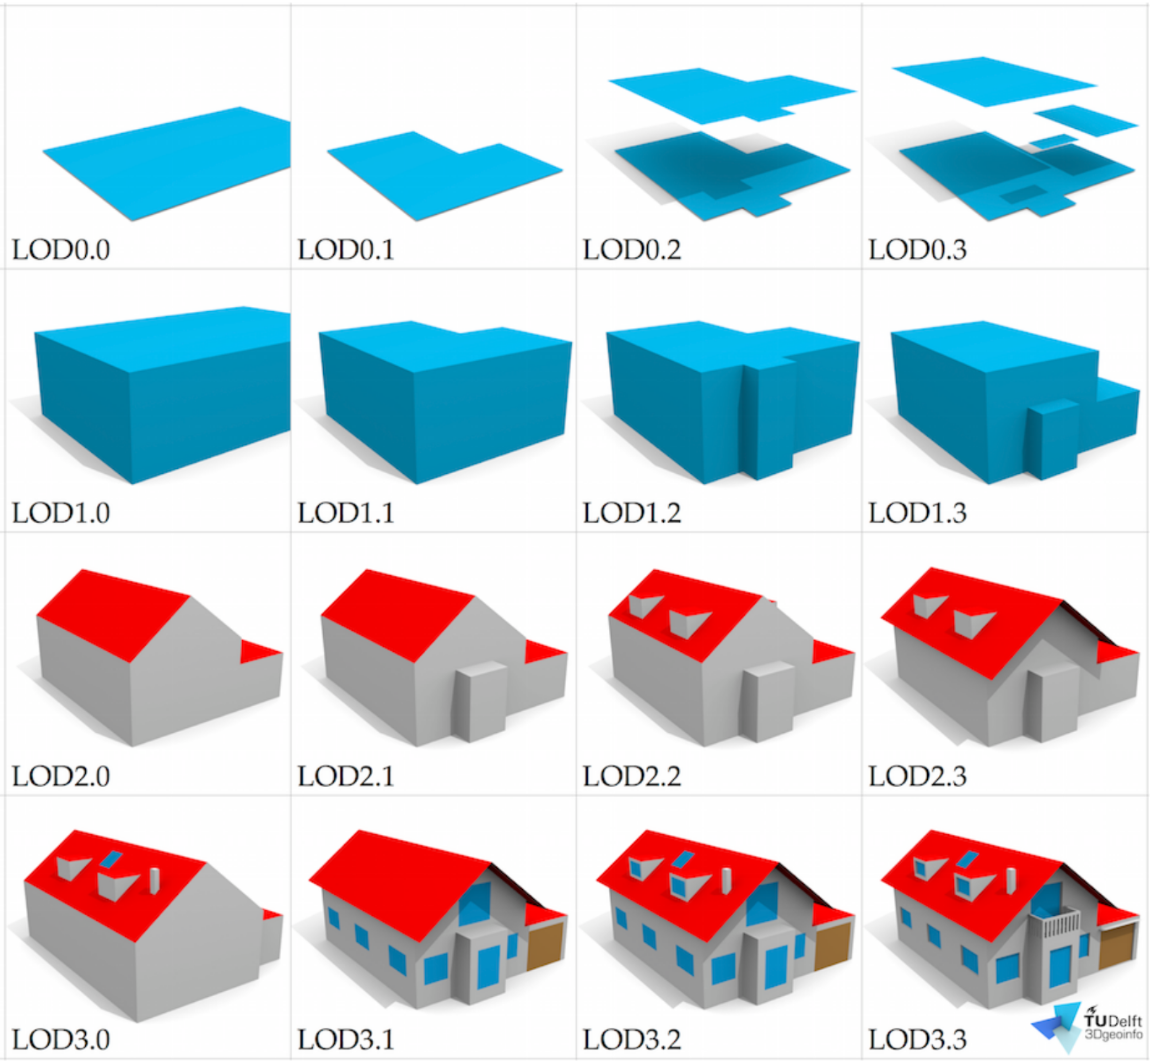
\includegraphics[keepaspectratio]{figures/chap_5_fig_2_improved_LOD_specification_for_3D_building_models.png}}

figure 3: Improved LOD specification for 3D building models \footnote{Biljecki,
  F., Ledoux, H., \& Stoter, J. (2016).}

\pandocbounded{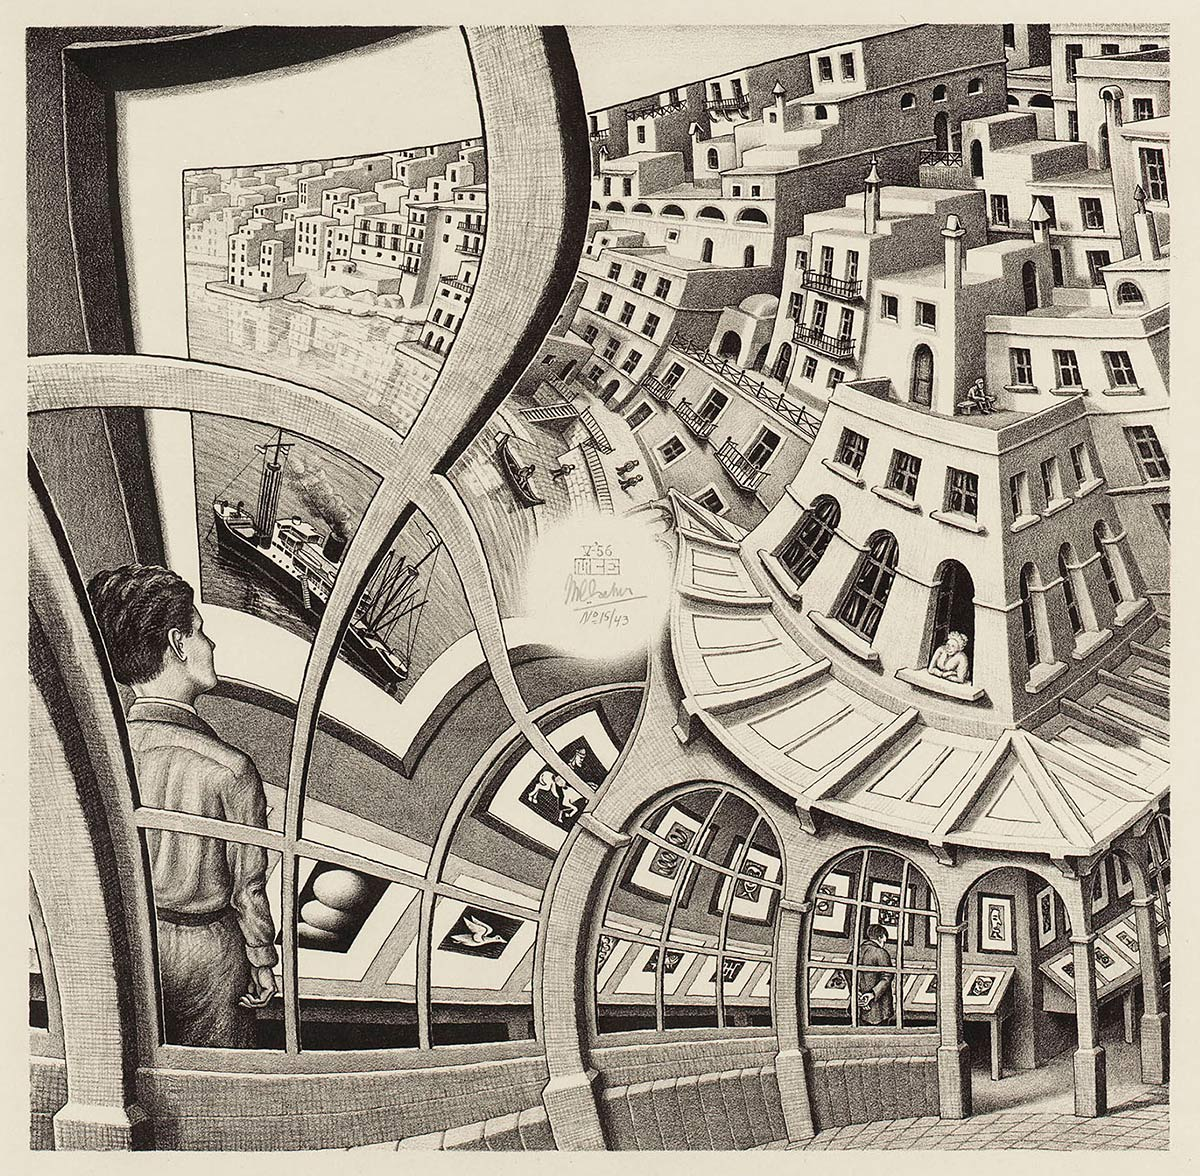
\includegraphics[keepaspectratio]{figures/chap_5_fig_4_Prentententoonstelling_escher.jpg}}

figure 4: The City of the Captive Globe, New York, 1972 \footnote{Rem
  Koolhaas \& Madelon Vriesendorp (1972).}

Parallel to this scientification of the built environment, other
disciplines were also severely favoured when facing the change in the
scale of the city, thanks to scientific and technological developments.
Geography had previously dealt for centuries with the scale of the
planet through the geodesic enterprise. This endeavour relied
increasingly on the XX century, on concrete representations taken from
aerial perspectives. This process culminated during the second half of
the century when satellite imaging allowed for the concrete
representation of the Earth at multiple scales.

Geodesy, derived from the Greek term for `division of the Earth,' is the
project responsible for measuring and producing an exact image of the
globe. A daughter of geography, cartography, and mathematics, geodesy
leaves behind the ancient, lived toponymic approach to location.
Instead, it constructs a system of localization based entirely on the
coordinates of the Earth's geometric copy: the geoid. Producing this
image of the world soon became a primary means of measuring our cities.
The sensory capture of global streets by technological giants like
Google pulled the aerial view of maps down to a closer representation of
our grounded experience.

The extension of the domain of the experimental disposition of the
geodesic enterprise, populated the global and local scales with remote
sensors. This marked an important advance on the concretization of the
image of the world, and a historical milestone of modern science. Though
not directly producing the physical urban environment, the geoid
introduced in the lives of modern citizens a continuous representation
of the Earth across every scale, from the cosmos down to the street. For
the first time in modern history, the citizen could visually access the
vast extension of the metropolis through a highly accurate virtual
surrogate.

Heidegger (1938) \footnote{Heidegger, M. (1977).} warned that the
abstract representation of the world would loom with its immensity over
our authentic sensible experience. Yet, with the execution of this
technological project, the image of the world has ironically become an
essential prosthetic technology for navigating the modern metropolis.
While this virtual mapping has changed neither the biological bandwidth
of our receptors nor the capacity of our effectors, its frictionless,
instantaneous locomotion has bypassed a major geographic barrier to
experience urban landscape. By effectively eliminating distances, this
technology simulates a return to the environmental scale.

As the modern epoch progresses, we are confronted with an image of the
world that represents the different aspects of the urban being in
increasingly higher degrees of resolution. This technospheric project
has not only limited itself to map the simple artifacts that compose the
city, but also has creept -increasingly evident in social networks
marketing- into the complex human aspects of the city.

Under a relationist framework (De Roo, 2016) \footnote{De Roo, G.
  (2016).}, the relations that we establish through a map of our world,
concretize an experience where humans are subjected to the cartographic
representation of urban beings. Mediated by an interface we sense and we
are sensed by the urban and its inhabitants. The concretization of this
image means that citizens and designers relate primarily to the
representation of the urban landscape, and then its physical
environment, in turn, is reconfigured to align with its images.

The extension of the geodesic project's domain to the representation of
the positions and relations of humans in space, pushes the enterprise
further in the technological concretisation of the horizon of our
experience. Although integrating human complexity into the geodesic
project remains theoretically controversial---a tension stemming from
the alienation inherent in disembodied habitation---the modern
scientific enterprise continuously seeks to concretize the habitation of
this image and develop a genealogy of its modification. While we march
towards the development of a remote sense of the urban landscape, we
surpass the spatial immensity of the city. Nonetheless, the lack of an
increase in our cognitive capacity to process this immense data,
combined with the absence of tools necessary to effectively act upon
this image of the world, constitutes the remaining frontier to the human
habitation of the modern megalopolis.

Index

Chapter 1

Chapter 2

Chapter 3

Chapter 4

Chapter 5

Chapter 6

References

Footnotes

\bookmarksetup{startatroot}

\chapter{A Genealogy of Machines to Inhabit the
World}\label{a-genealogy-of-machines-to-inhabit-the-world}

\bookmarksetup{startatroot}

\chapter{\texorpdfstring{{/06} A Genealogy of Machines to Inhabit the
World}{/06 A Genealogy of Machines to Inhabit the World}}\label{a-genealogy-of-machines-to-inhabit-the-world-1}

While remote sensing eliminates locomotion as a variable---compressing
spatial immensity into an instant---it reveals another critical
cognitive limitation issued from immensity. The primary barrier to
navigating the modern urban landscape shifts to the information
bandwidth of the human observer; as Portugali (2016) \footnote{Portugali,
  J. (2016).} notes, the sheer proliferation of spatial data overwhelms
the human capacity for internal representation.

To breach this other aspect of this ontological barrier, design
methodologies increasingly rely on technologies that assist in the
intake, compilation, and representation of environmental data. Robotic
agents and algorithmic systems have emerged as necessary cognitive
prosthetics, enabling simultaneous perception and action across a
multiplicity of spaces. Within the contemporary urban experience,
navigational agents, search engines, and AI chatbots already operate
with agentic behavior. Consequently, the immense urban landscape is
accessed not through direct intuition, but through the mediation of
mechanical messengers.

The design and concretization through agents situate the user in a
position where intent begins to be constituted and synthesized by the
messengers. The announcement delivered by the user is subsequently
processed by these messengers. Message delivery and the corresponding
response operate entirely through this delegated sensing. Consequently,
the concretization of design becomes the design of the messengers'
experience; these agents navigate every facet of the model, undergoing
the concrete experience within the design medium prior to its physical
concretization. The production and reproduction of the image of the
world constitutes an inhabited technological stratum. Because of the
sheer scale and dimensionality of this reality, it remains inaccessible
to the direct observation of the human designer. This virtual
surrogate---commercially concretized by platforms such as Nvidia's
`Omniverse'---is inhabited not only by the digital representations of
urban entities, but is actively navigated by the autonomous messengers
that relate to them.

The design medium operates as a blank canvas where the user's intentions
can be expressed in highly abstract forms, which are subsequently
interpreted by the messengers. The drafting table now accommodates
generalized traces; the scale and volume of information no longer
constitute a barrier, as the preliminary interpretation is executed
beforehand by the machine. This establishes a design medium
characterized by a double hermeneutic: first, the autonomous agents
interpret the human input and the digital material; second, the user
must interpret the resulting algorithmic synthesis.

At first glance, one might assume this technological paradigm elevates
the designer to an omnipotent position, transmitting teleological intent
strictly through mechanical messengers. This dynamic mirrors a
theological structure wherein an entity depends upon emissaries to
manifest within a spatial dimension it cannot physically inhabit---in
this instance, the sheer immensity of the geographic scale. However,
critical analysis reveals a structural inversion: as these messengers
develop and concretize within the urban environment, they cease to be
mere conduits and become our habitats. As human interaction pours into
these systems, the relational hierarchy inverts; the algorithmic
infrastructure envelopes the citizen, emerging as a transcendental urban
being that dictates the terms of modern habitation.

This inversion establishes a perichoresis---a mutual intertwining
between human and machine to inhabit the world. Analyzed through
Capurro's (2003) \footnote{Capurro, R. (2003).} angeletics, the
mechanics of these messengers dictate that they do not merely transmit
human intent; they actively configure the human subject's perception
just as the human configures their algorithms.

This reciprocal configuration ultimately necessitates a transition
toward an animistic view of the city. As autonomous agents continuously
process, translate, and act upon the urban tissue, the inert
infrastructure of the megalopolis is endowed with a cybernetic vitality.
Drawing upon Emanuele Coccia's (2021) \footnote{Coccia, E. (2021).}
theoretical framework, these algorithmic messengers function as
contemporary ``philosopher's stones''---alchemical mediums that animate
the previously inanimate material of the metropolis. Through this
angeletic infrastructure, the urban landscape ceases to be a static,
geographic object and becomes an animistic ecology, defined by a
continuous, communicative metabolism between human intent and autonomous
matter.

figure 1: NVIDIA Omniverse Foundational Technology Montage I GTC Spring
2025 Edition \footnote{NVIDIA. (2025).}

\pandocbounded{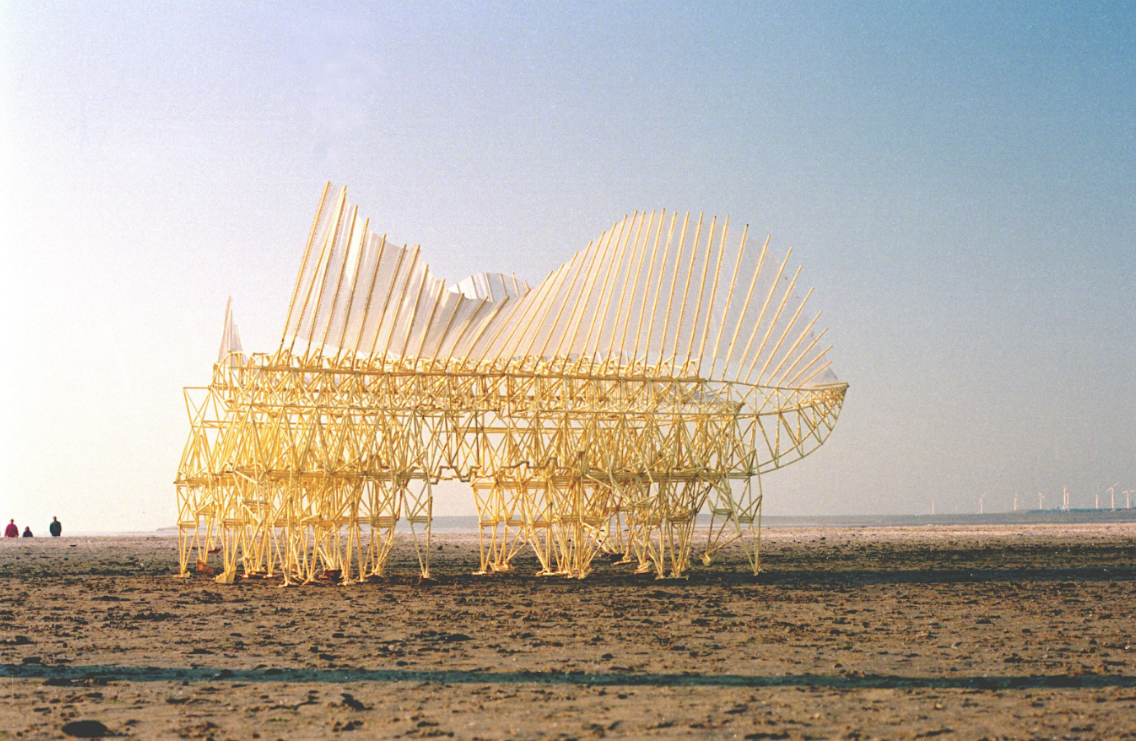
\includegraphics[keepaspectratio]{figures/chap_6_fig_2_currens_ventosa_oostvoorne_NL_1993_photo_adriaan_Kok.png}}

figure 2: Currens Ventosa, Oostvoorne NL 1993, photo: Adriaan Kok
\footnote{Currens Ventosa, Oostvoorne.}

\pandocbounded{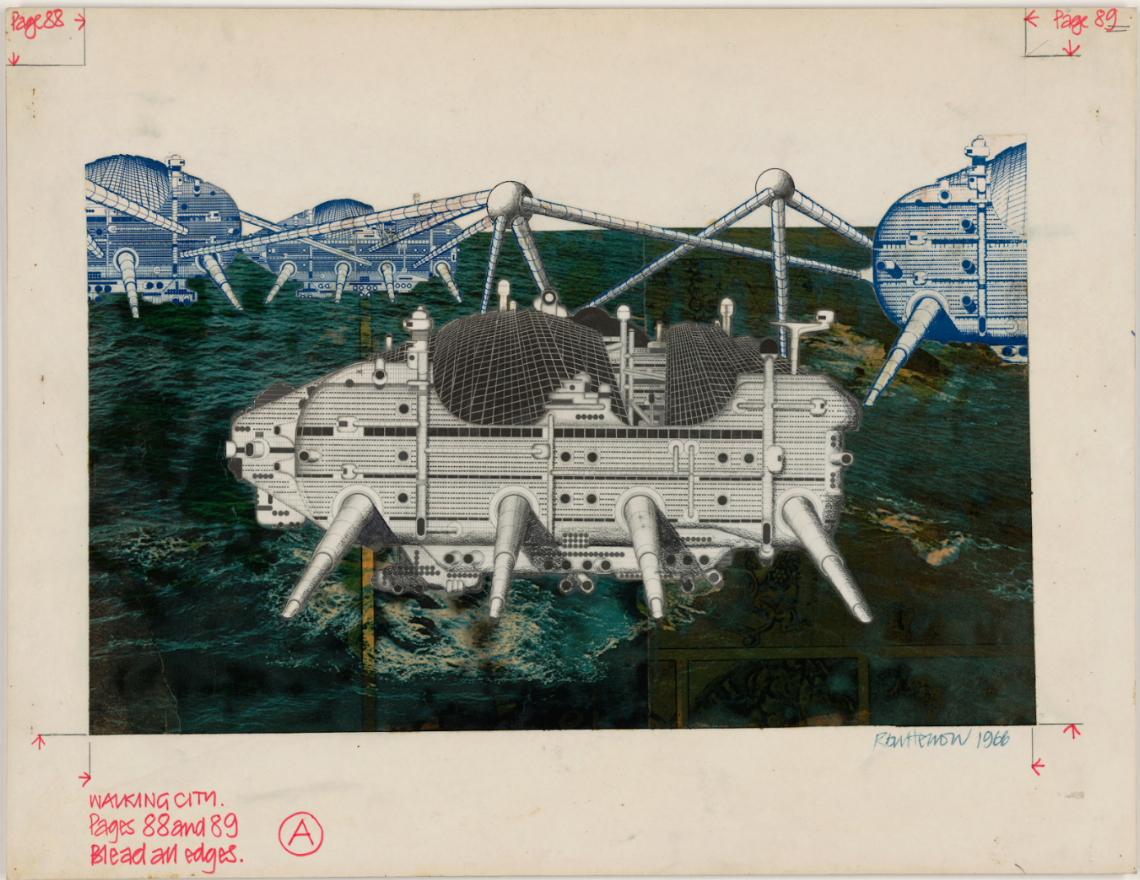
\includegraphics[keepaspectratio]{figures/chap_6_fig_3_ron_herron_walking_city_on_the_ocean_project_exterior_perspective_1966.png}}

figure 3: Ron Herron Walking City on the Ocean, project (Exterior
perspective) 1966 \footnote{Ron Herron (1966).}

Index

Chapter 1

Chapter 2

Chapter 3

Chapter 4

Chapter 5

Chapter 6

References

Footnotes

\bookmarksetup{startatroot}

\chapter{References \& Bibliography}\label{references-bibliography}

{/REF} References

The City of the Captive Globe

\subsection{Text Citations}\label{text-citations}

\begin{itemize}
\tightlist
\item
  Portugali, J. (2016). What Makes Cities Complex? In J. Portugali \& E.
  Stolk (Eds.), \emph{Complexity, Cognition, Urban Planning and Design}
  (pp.~3--19). Springer International Publishing.
\item
  Stolk, E., \& Portugali, J. (2016). A Complexity-Cognitive View on
  Scale in Urban Design. In J. Portugali \& E. Stolk (Eds.),
  \emph{Complexity, Cognition, Urban Planning and Design}
  (pp.~217--252). Springer International Publishing.
\item
  Kant, I. (1998). \emph{Critique of pure reason} (P. Guyer \& A. W.
  Wood, Trans.). Cambridge University Press. (Original work published
  1781)
\item
  Fondation Gabriel Péri. (2022, April 21). \emph{Éric Puisais, Henri
  Lefebvre, une philosophie de la géographie} {[}Video{]}. YouTube.
\item
  Koolhaas, R. (1995). Bigness, or the Problem of Large. In R. Koolhaas
  \& B. Mau (Eds.), \emph{S,M,L,XL} (pp.~495--516). The Monacelli Press.
\item
  Lefebvre, H. (1972). \emph{Urbanose: Entretien avec Henri Lefebvre}
  {[}Documentary{]}. Office National du Film du Canada.
\item
  De Roo, G. (2016). Framing the Planning Game: A Cognitive
  Understanding of the Planner's Rationale in a Differentiated World. In
  J. Portugali \& E. Stolk (Eds.), \emph{Complexity, Cognition, Urban
  Planning and Design} (pp.~173--199). Springer International
  Publishing.
\item
  Kousoulas, S., \& Radman, A. (2026). Annotate This! Semiotisation,
  Automation and the Recursive Causality of Images. In A. Biglari (Ed.),
  \emph{Open Semiotics} (Vol. 5).
\item
  Koolhaas, R. (2002). Junkspace. \emph{October}, 100, 175--190.
\item
  von Uexküll, J. (1957). A stroll through the worlds of animals and
  men: A picture book of invisible worlds (C. H. Schiller, Trans.). In
  C. H. Schiller (Ed.), \emph{Instinctive behavior: The development of a
  modern concept} (pp.~5--80). International Universities Press.
  (Original work published 1934)
\item
  Aristotle. (1984). \emph{Metaphysics} (W. D. Ross, Trans.). In J.
  Barnes (Ed.), \emph{The complete works of Aristotle: The revised
  Oxford translation} (Vol. 2, pp.~1552--1728). Princeton University
  Press. (Original work published ca. 350 B.C.E.)
\item
  Heidegger, M. (1977). The age of the world picture. In W. Lovitt
  (Trans.), \emph{The question concerning technology and other essays}
  (pp.~115--154). Harper \& Row. (Original work published 1950)
\item
  Simondon, G. (2017). \emph{On the mode of existence of technical
  objects} (C. Malaspina \& J. Rogove, Trans.). Univocal Publishing.
  (Original work published 1958)
\item
  Sloterdijk, P. (2016). \emph{Foams: Spheres volume III: Plural
  spherology} (W. Hoban, Trans.). Semiotext(e). (Original work published
  2004).
\item
  Le Corbusier. (1923). \emph{Vers une architecture}. G. Crès et Cie.
\item
  Fabian Alvarado David. (2016, 7 juillet). \emph{Le mouvement dans les
  sociétés hypermodernes François Ascher} {[}Vidéo{]}. YouTube.
\item
  Capurro, R. (2003). \emph{Angeletics - A message theory}. Rafael
  Capurro.
\item
  Coccia, E. (2021). \emph{Filosofia della casa: Lo spazio domestico e
  la felicità}. Einaudi.
\end{itemize}

\subsection{Image Citations}\label{image-citations}

\begin{itemize}
\tightlist
\item
  Uhl, Johannes H.: Animating 200 years of urban spatial development in
  35 U.S. cities. Copernicus Publications, 2020.
\item
  United Nations, Department of Economic and Social Affairs, Population
  Division. (2019). \emph{World urbanization prospects}
\item
  Zhu, X. X., Chen, S., Zhang, F., Shi, Y., and Wang, Y.:
  GlobalBuildingAtlas: an open global and complete dataset of building
  polygons, heights and LoD1 3D models, Earth Syst. Sci. Data, 17,
  6647--6668, 2025.
\item
  von Uexküll, J. (1957). A stroll through the worlds of animals and
  men: A picture book of invisible worlds. In C. H. Schiller (Ed. \&
  Trans.), \emph{Instinctive behavior: The development of a modern
  concept} (pp.~5--80). International Universities Press. (Original work
  published 1934)
\item
  \emph{Blind men and the elephant} {[}Illustration{]}. (1907). In
  \emph{The Heath readers by grades} (p.~69). D.C. Heath and Company.
\item
  Stolk, E., \& Portugali, J. (2016). A Complexity-Cognitive View on
  Scale in Urban Design. In J. Portugali \& E. Stolk (Eds.),
  \emph{Complexity, Cognition, Urban Planning and Design}
  (pp.~217--252). Springer International Publishing.
\item
  Eisen, C. (1755). \emph{Frontispiece} {[}Engraving{]}. In M.-A.
  Laugier, \emph{Essai sur l'architecture} (2nd ed.). Duchesne.
\item
  Le Corbusier. (1914). \emph{Maison Dom-Ino, elevation/perspective
  view} {[}Architectural Drawing{]}. Fondation Le Corbusier, Paris,
  France.
\item
  Levittown library. (1950). Early Capes Aerial View of Levittown.
\item
  SITE (1981), \emph{Highrise of houses}.
\item
  Sharpsteen, B. (Director). (1938). \emph{Mickey's trailer} {[}Film{]}.
  Walt Disney Productions.
\item
  Ed Ruscha (1966), \emph{Standard Station}
\item
  Shuttle Nasa Topography Mission (SRTM) (1999)
\item
  Google Earth. (2018, December 7). \emph{Google Earth Studio -
  Animation Reel} {[}Video{]}. YouTube.
\item
  Biljecki, F., Ledoux, H., \& Stoter, J. (2016). An improved LOD
  specification for 3D building models. \emph{Computers, Environment and
  Urban Systems}, 59, 25--37.
\item
  Rem Koolhaas \& Madelon Vriesendorp, \emph{The City of the Captive
  Globe}, New York, 1972. Gouache and pencil on paper, 318 × 441 mm. The
  Museum of Modern Art, New York.
\item
  NVIDIA. (2025, March 24). \emph{NVIDIA Omniverse Foundational
  Technology Montage I GTC Spring 2025 Edition} {[}Video{]}. YouTube.
\item
  Currens Ventosa, Oostvoorne NL 1993, photo: Adriaan Kok
\item
  Ron Herron \emph{Walking City on the Ocean}, project (Exterior
  perspective) 1966
\end{itemize}

Index

Chapter 1

Chapter 2

Chapter 3

Chapter 4

Chapter 5

Chapter 6

References




\end{document}
